Yanee is a bird enthusiast. Since reading about \textit{IP over Avian Carriers} (IPoAC), she has spent much of her time training a flock of intelligent parrots to carry messages over long distances.

Yanee's dream is to use her birds to send a message $M$ to a land far far away. Her message $M$ is a
sequence of $N$ (not necessarily distinct) integers, each between $0$ and $255$, inclusive. Yanee keeps
$K$ specially-trained parrots. All the parrots look the same; Yanee cannot tell them apart. Each bird
can remember a single integer between $0$ and $R$, inclusive.

Early on, she tried a simple scheme: to send a message, Yanee carefully let the birds out of the
cage one by one. Before each bird soared into the air, she taught it a number from the message sequence in order. Unfortunately, this scheme did not work. Eventually, all the birds did arrive at
the destination, but they did not necessarily arrive in the order in which they left. With this
scheme, Yanee could recover all the numbers she sent, but she was unable to put them into the
right order.

To realize her dream, Yanee will need a better scheme, and for that she needs your help. Given a
message $M$, she plans to let the birds out one by one like before. She needs you to write a program that will perform two separate operations:
\begin{itemize}
\item First, your program should be able to read a message $M$ and transform it into a sequence
of at most $K$ integers between $0$ and $R$ that she will teach the birds.
\item Second, your program should be able to read the list of integers between $0$ and $R$ received
as the birds reach their destination, and then transform it back to the original message $M$.
\end{itemize}
You may assume that all parrots always arrive at the destination, and that each of them remembers the number it was assigned. Yanee reminds you once again that the parrots may arrive in
any order. Note that Yanee only has $K$ parrots, so the sequence of integers between $0$ and $R$ that
you produce must contain at most $K$ integers.

Your task is to write two separate procedures. One of them will be used by the sender (encoder) and the other by
the receiver (decoder).

The overall process is shown in the following figure.

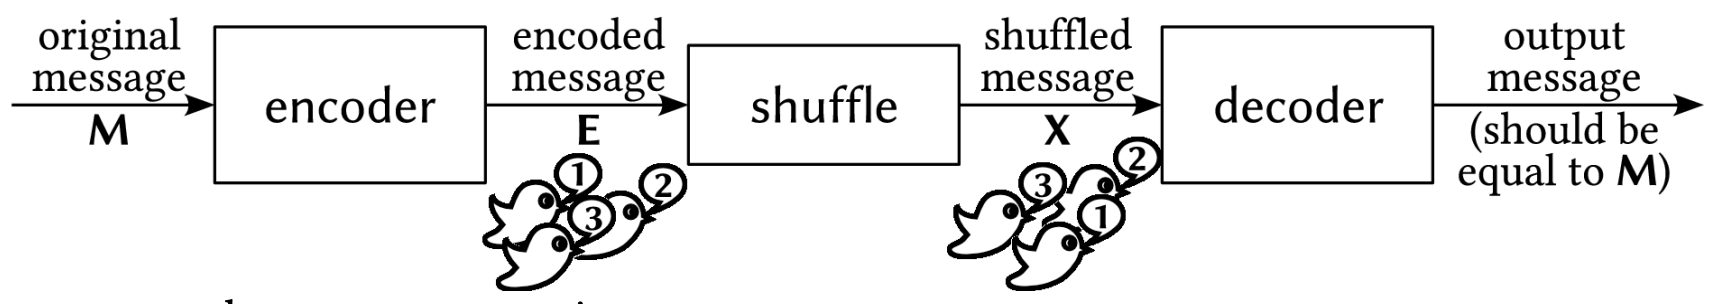
\includegraphics[width=175mm]{parrots1.png}

The two procedures you are to write are:
\begin{itemize}
\item Procedure \t{encode(N,M)} that takes the following parameters:
\begin{itemize}
\item $N$~--- the length of the message.
\item $M$~--- a one-dimensional array of $N$ integers representing the message. You may assume that $0 \leq M[i] \leq 255$ for $0 \leq i < N$.
\end{itemize}
This procedure must encode the message $M$ into a sequence of integers between $0$ and $R$,
inclusive, that shall be sent using the parrots. To report this sequence, your procedure
\t{encode} must call the procedure \t{send(a)} for each integer $a$ that you wish to give to one of
the birds.
\item Procedure \t{decode(N,L,X)} that takes the following parameters:
\begin{itemize}
\item $N$~--- the length of the original message.
\item $L$~--- the length of the message received (the number of birds that were sent).
\item $X$~--- a one-dimensional array of $L$ integers representing the received numbers. The
numbers $X[i]$ for $0 \leq i < L$ are precisely the numbers that your procedure encode
produced, but possibly rearranged into a different order.
\end{itemize}
This procedure must recover the original message. To report it, your procedure \t{decode}
must call the procedure \t{output(b)} for each integer $b$ in the decoded message, in the correct order.
\end{itemize}
Note that $R$ and $K$ are not given as input parameters~--- please see the subtask descriptions below.
In order to correctly solve a given subtask, your procedures must satisfy the following conditions:
\begin{itemize}
\item All integers sent by your procedure \t{encode} must be in the range specified in the subtask.
\item The number of times your procedure \t{encode} calls the procedure \t{send} must not exceed
the limit $K$ specified in the subtask. Please note that $K$ depends on the length of the message.
\item Procedure \t{decode} must correctly recover the original message $M$ and call the procedure
\t{output(b)} exactly $N$ times, with $b$ equal to $M[0], M[1], \dots, M[N-1]$, respectively.
\end{itemize}
In the last subtask, your score varies according to the ratio between the lengths of the encoded
message and the original message.

